\documentclass[letterpaper,11pt]{article}
\oddsidemargin -1.0cm \textwidth 17.5cm

\usepackage[utf8]{inputenc}
\usepackage[activeacute,spanish, es-lcroman]{babel}
\decimalpoint
\usepackage{amsfonts,setspace}
\usepackage{amsmath}
\usepackage{amssymb, amsmath, amsthm}
\usepackage{comment}
\usepackage{float}
\usepackage{amssymb}
\usepackage{dsfont}
\usepackage{anysize}
\usepackage{multicol}
\usepackage{enumerate}
\usepackage{graphicx}
\usepackage[left=1.5cm,top=2cm,right=1.5cm, bottom=1.7cm]{geometry}
\setlength\headheight{1.5em} 
\usepackage{fancyhdr}
\usepackage{multicol}
\usepackage{hyperref}
\usepackage{wrapfig}
\usepackage{subcaption}
\usepackage{siunitx}
\usepackage{cancel}
\usepackage{mdwlist}
\usepackage{svg}
\usepackage{tcolorbox}
\pagestyle{fancy}
\fancyhf{}
\renewcommand{\labelenumi}{\normalsize\bfseries P\arabic{enumi}.}
\renewcommand{\labelenumii}{\normalsize\bfseries (\alph{enumii})}
\renewcommand{\labelenumiii}{\normalsize\bfseries \roman{enumiii})}


\begin{document}

\fancyhead[L]{\itshape{Facultad de Ciencias F\'isicas y Matem\'aticas}}
\fancyhead[R]{\itshape{Universidad de Chile}}

\begin{minipage}{11.5cm}
    \begin{flushleft}
        \hspace*{-0.6cm}\textbf{FI1000-1 Introducción a la Física Clásica}\\
        \hspace*{-0.6cm}\textbf{Profesora:} Jocelyn Dunstan\\
        \hspace*{-0.6cm}\textbf{Auxiliar:} Alejandro Silva\\
        \hspace*{-0.6cm}\textbf{Ayudantes:} Macarena Muñoz \& Catalina Vargas\\
    \end{flushleft}
\end{minipage}

\begin{picture}(2,3)
    \svgpath{../}  % descomentar si se agrega a carpeta "auxiliares"/"ejercicios"
    \put(366, 10){\includesvg[scale=0.31]{img/dfi.svg}}
\end{picture}

\begin{center}
    \tiny{último}
	\LARGE\textbf{Auxiliar \#14:}\\
	\Large{Hidrostática e Hidrodinámica}
\end{center}

\vspace{-1cm}
\begin{enumerate}\setlength{\itemsep}{0.4cm}

\rfoot[]{pág. \thepage}

\item[]

\item
\begin{multicols}{2}
    Un cubo de madera de longitud $H$ flota en la interfaz entre aceite y agua con su superficie inferior a una distancia $h$ de la interfaz. Si la densidad del aceite es $\rho_{a}$ y la densidad del agua es $\rho_{w}$
    
        \begin{enumerate}
            \item Determine la presión manométrica en la superficie superior e inferior del bloque
            \item Determine la densidad y la masa del bloque 
        \end{enumerate}
    
    \columnbreak
    
    \begin{figure}[H]
        \centering
        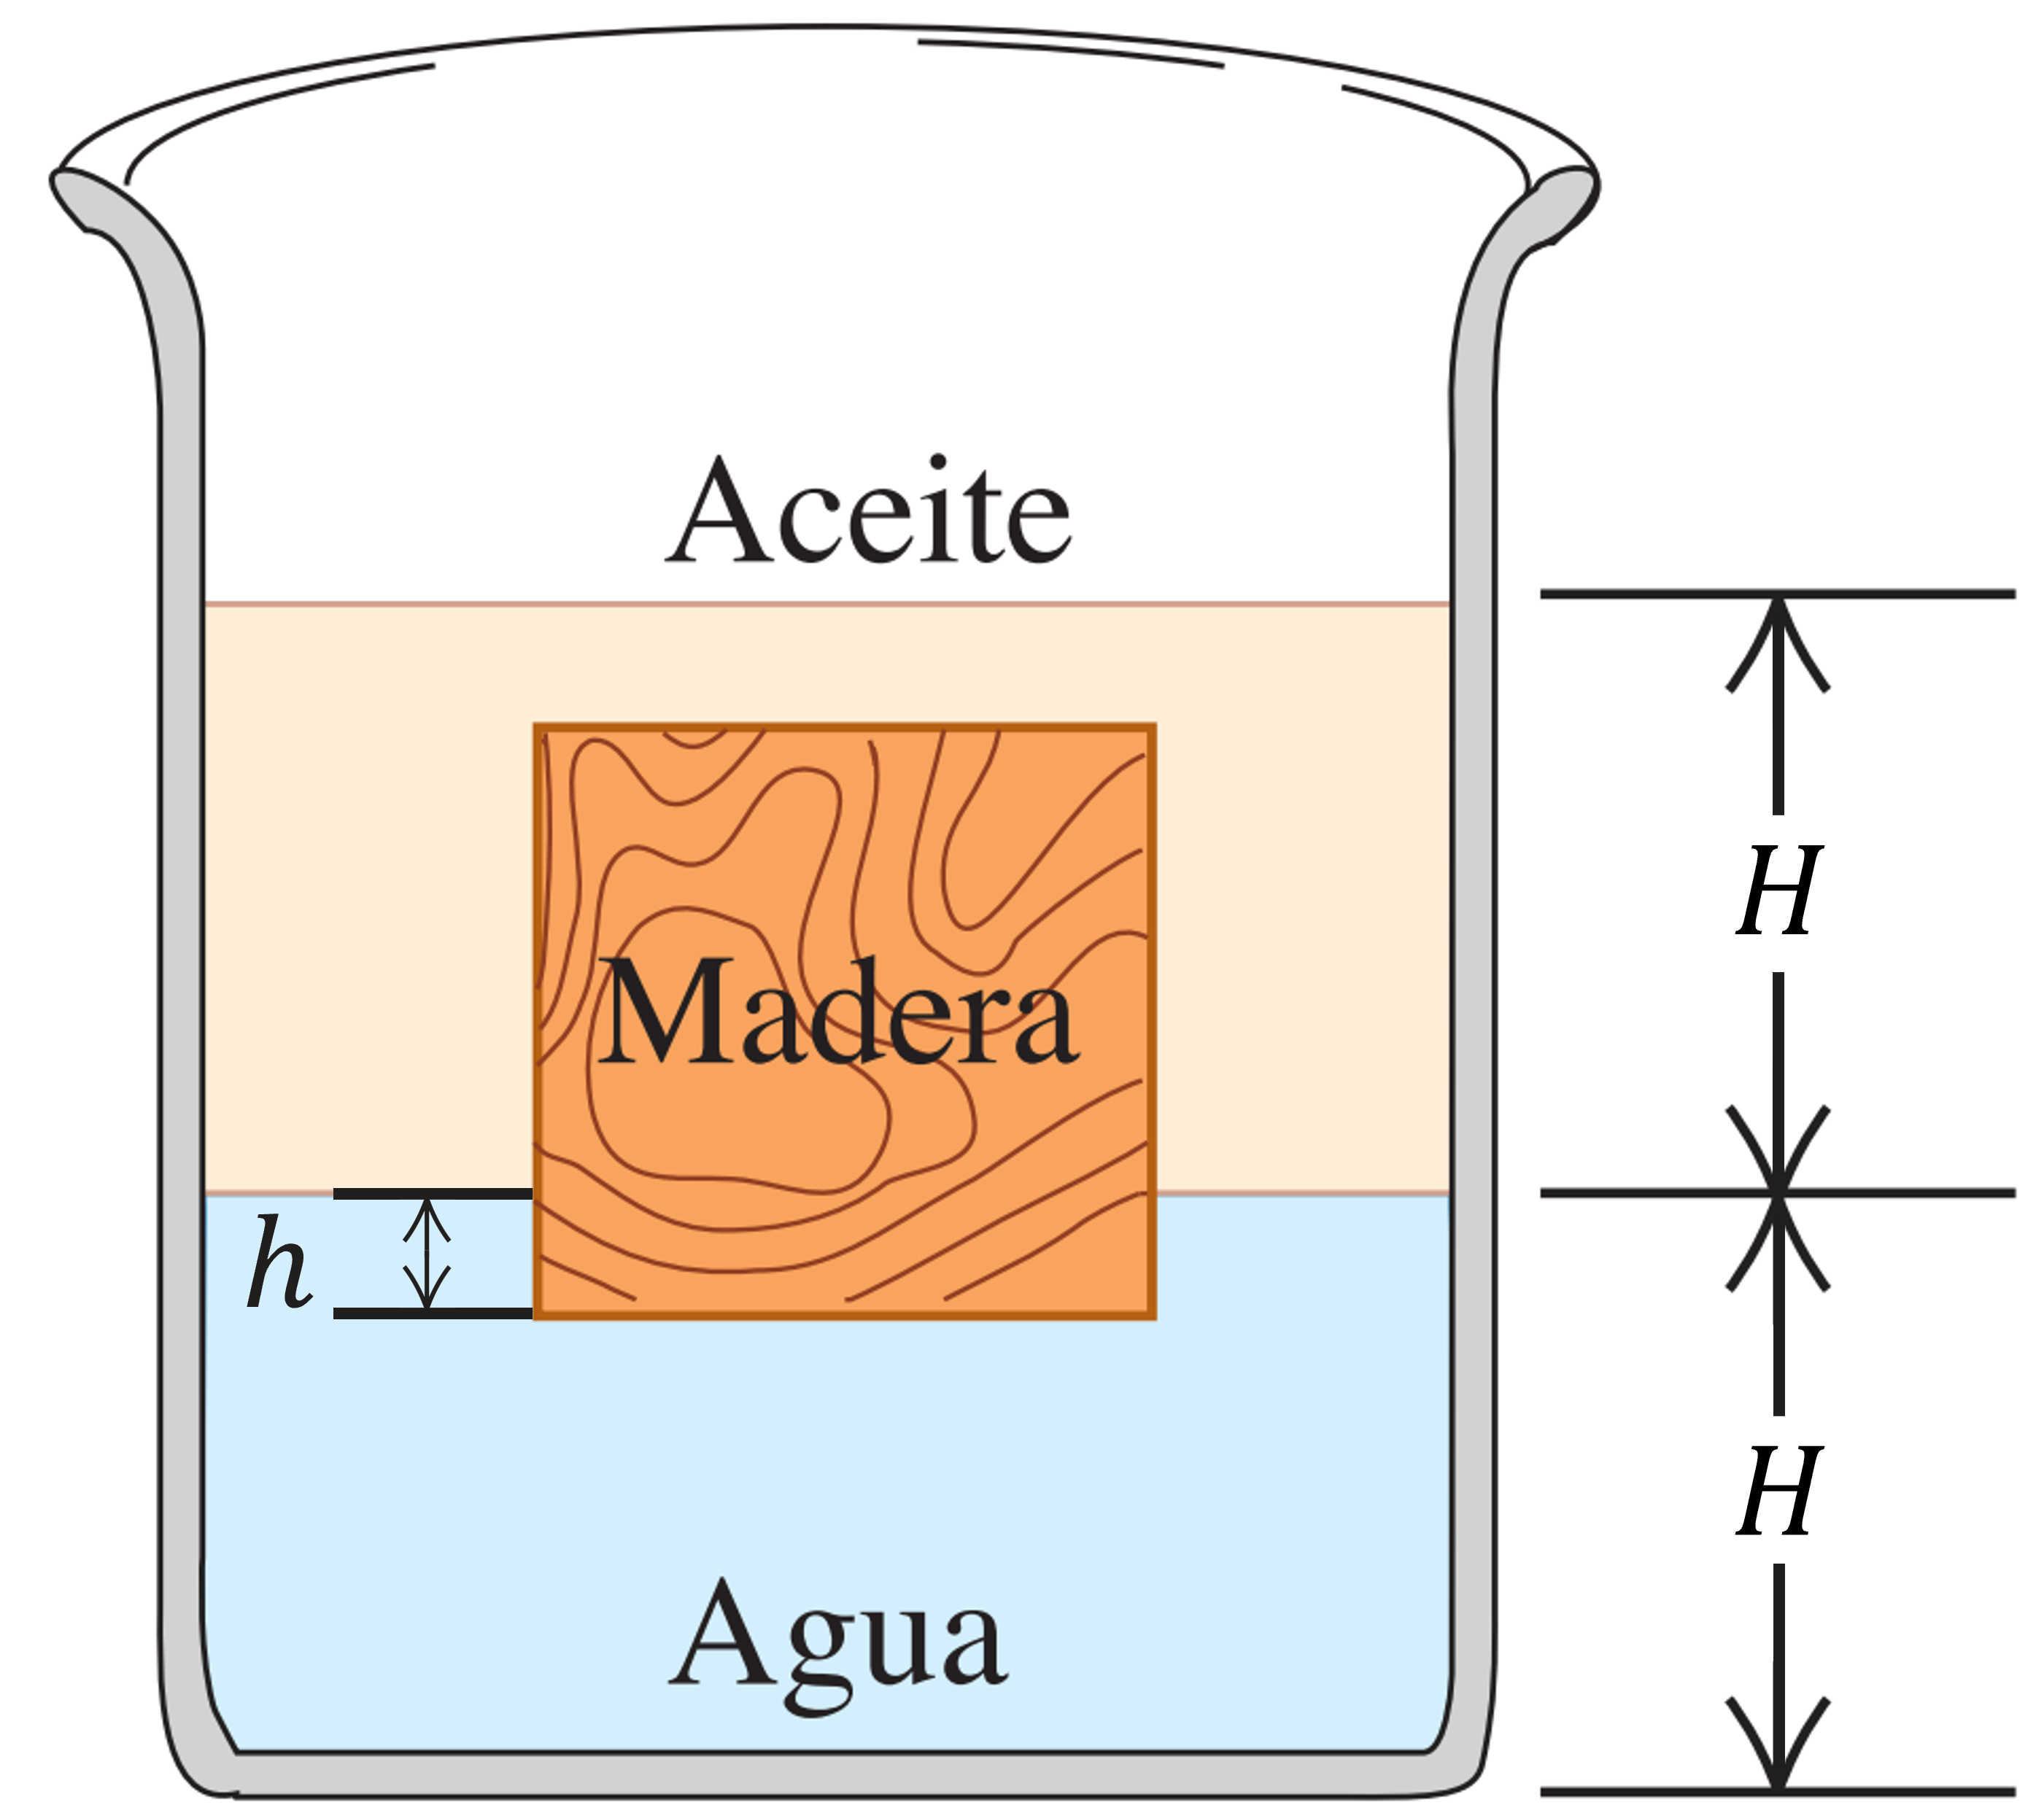
\includegraphics[width=0.45\linewidth]{2021-2/img/aux14/cubo-madera.png}
    \end{figure}
\end{multicols}

\item
\begin{multicols}{2}
    Dos globos esféricos inflados con un gas incompresible de densidad $\rho_g$, ambos de radio $R$, se unen mediante una cuerda de longitud $L$. Los dos globos se mantienen bajo el agua con el punto medio de la cuerda fijo al fondo. Calcular la fuerza de contacto entre los globos.
    
    \columnbreak
    
    \begin{figure}[H]
        \centering
        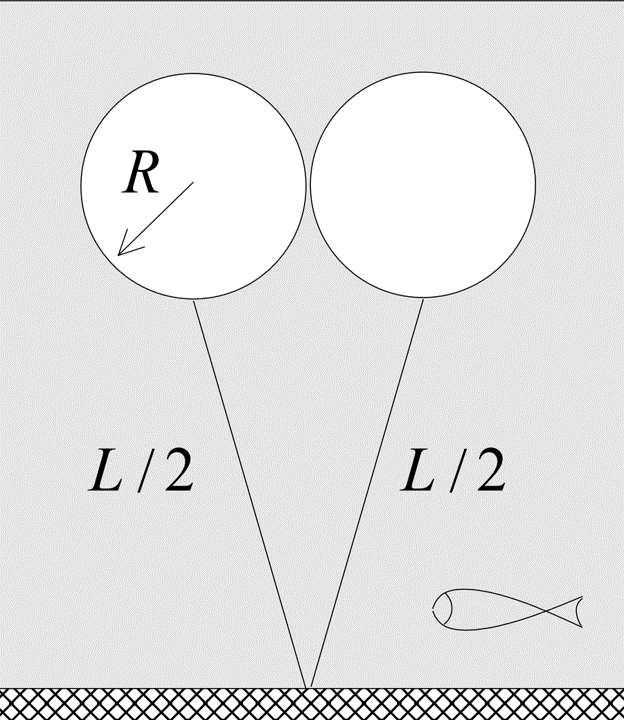
\includegraphics[height=0.4\linewidth]{2021-2/img/aux14/globos.png}
    \end{figure}
\end{multicols}

\item 
\begin{multicols}{2}
    Suponga que el nivel de un líquido (agua) en un tambor tiene una altura $h$. A una altura $b$ se hace una pequeña perforación lateral que permite que el agua emerja horizontalmente. ¿A qué altura debe hacerse la perforación para que el alcance $d$ del agua sea máximo?
    
    \columnbreak
    
    \begin{figure}[H]
        \centering
        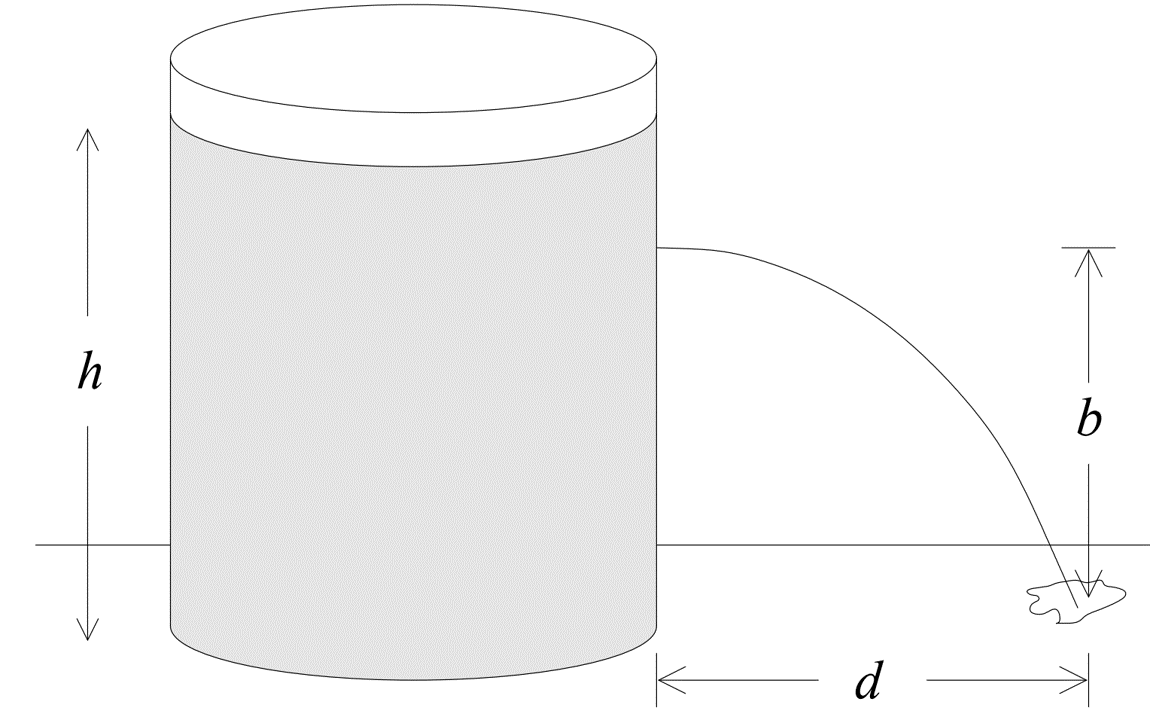
\includegraphics[width=0.55\linewidth]{2021-2/img/aux14/tambor.png}
    \end{figure}
\end{multicols}

\item Un tubo horizontal por el que fluye líquido de densidad $\rho_0$ a razón de $Q$~$\SI{}{\meter^3\per\second}$, se bifurca en dos ramas en el plano vertical, una superior y otra inferior, de secciones transversales $a_1=a_2=a$, abiertas a la atmósfera. Si la distancia entre las ramas es $h$, determine:
    \begin{enumerate}
        \item Las cantidades $q_1$ y $q_2$ de líquido (en $\SI{}{\meter^3\per\second}$) que fluyen por ambas ramas
        \item La condición que debe cumplir $Q$ para que haya flujo en la rama superior
    \end{enumerate}
    
    \begin{figure}[H]
        \centering
        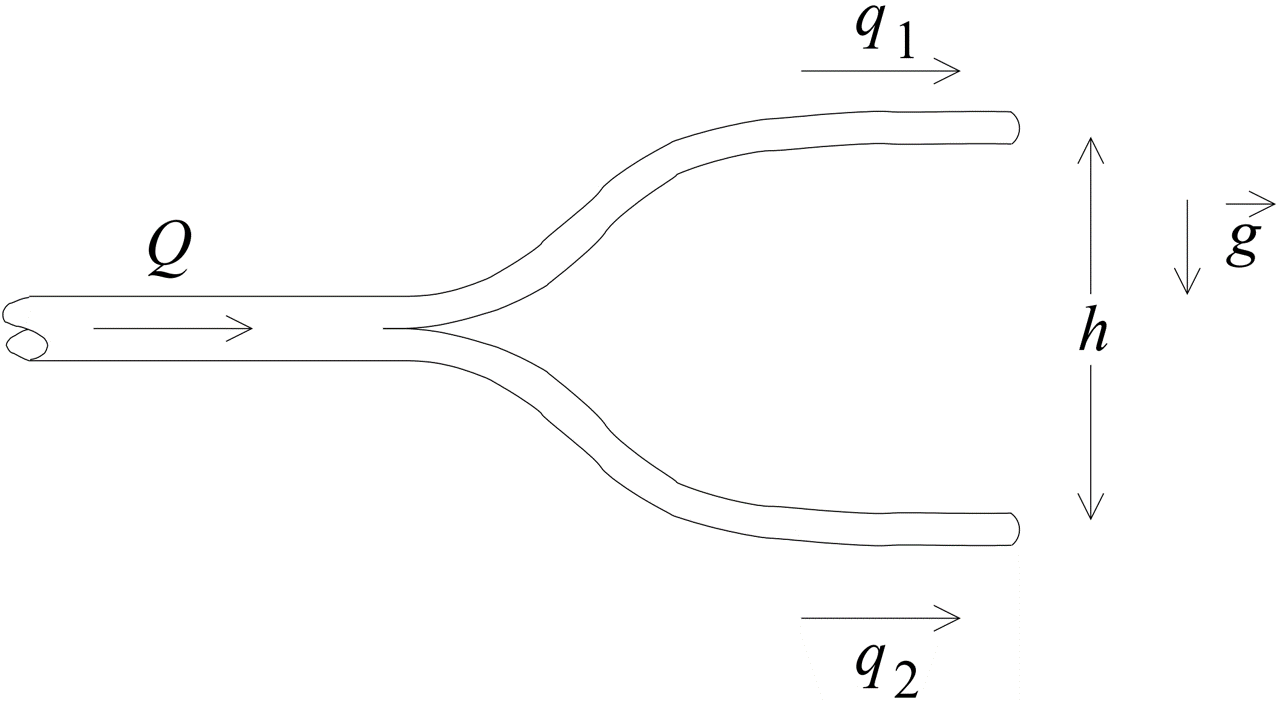
\includegraphics[width=0.3\linewidth]{2021-2/img/aux14/y.png}
    \end{figure}



% ---------------
% Recordatorios:
% --------------
% 1. \begin{multicols}{2} -> 2 columnas, acepta texto e imagen
% 2. \begin{figure} / \begin{subfigure}[t]{0.45\textwidth}
% 3. Para imágenes vectoriales con texto en LaTeX 
%   \begin{figure}[htbp]
%       \centering
%       \svgpath{../Imagenes/ejercicios}  -> el ".." para irse pa'trás 
%       \includesvg{ej5.svg}
%   \end{figure}
% 4. \linewidth (ancho de línea) and \baselineskip (alto de línea)
\end{enumerate}
\end{document}